\documentclass[conference]{IEEEtran}
\IEEEoverridecommandlockouts
% The preceding line is only needed to identify funding in the first footnote. If that is unneeded, please comment it out.
\usepackage{cite}
\usepackage{amsmath,amssymb,amsfonts}
\usepackage{algorithmic}
\usepackage{graphicx}
\usepackage{textcomp}
\usepackage{xcolor}
\usepackage{listings}
\usepackage{xcolor}
\usepackage{subcaption}

\lstset{
    language=Python,
    basicstyle=\ttfamily\small,
    keywordstyle=\color{blue},
    commentstyle=\color{gray},
    stringstyle=\color{red},
    frame=single,
    breaklines=true,
    showstringspaces=false
}


\def\BibTeX{{\rm B\kern-.05em{\sc i\kern-.025em b}\kern-.08em
    T\kern-.1667em\lower.7ex\hbox{E}\kern-.125emX}}

\title{Colorization of Grayscale Images\\
}

\makeatletter
\newcommand{\newlineauthors}{%
  \end{@IEEEauthorhalign}\hfill\mbox{}\par
  \mbox{}\hfill\begin{@IEEEauthorhalign}
}
\makeatother

\author
{\IEEEauthorblockN{Buddhika Ariyarathna}
\IEEEauthorblockA{\textit{Department of Computer Engineering} \\
\textit{University of Peradeniya} \\
Sri Lanka \\
e20024@eng.pdn.ac.lk}
\and
\IEEEauthorblockN{Kavindu Methpura}
\IEEEauthorblockA{\textit{Department of Computer Engineering} \\
\textit{University of Peradeniya} \\
Sri Lanka \\
e20254@eng.pdn.ac.lk}
\and
\IEEEauthorblockN{Bhagya Senavirathna}
\IEEEauthorblockA{\textit{Department of Computer Engineering} \\
\textit{University of Peradeniya} \\
Sri Lanka \\
e20366@eng.pdn.ac.lk}
\newlineauthors
\IEEEauthorblockN{Amanda Siriwardane}
\IEEEauthorblockA{\textit{Department of Computer Engineering} \\
\textit{University of Peradeniya} \\
Sri Lanka \\
e20378@eng.pdn.ac.lk}
\and
\IEEEauthorblockN{Janith Wanasinghe}
\IEEEauthorblockA{\textit{Department of Computer Engineering} \\
\textit{University of Peradeniya} \\
Sri Lanka \\
e20420@eng.pdn.ac.lk}
}
\begin{document}
\maketitle

\begin{abstract}

Colorization of grayscale images is a challenging problem with applications in image restoration, medical imaging, and digital arts. Traditional methods, including spatial and frequency domain transformations, often struggle with seamless color assignment and perceptual consistency. This project integrates classical image processing techniques with deep learning to enhance grayscale-to-color image translation.

Initially, intensity-based segmentation, Fourier domain processing, and heuristic color mapping were implemented. However, these approaches had limitations in structural detail preservation and natural color transitions. To improve performance, a hybrid Convolutional Neural Network (CNN)-based framework was introduced, constructed by integrating various components from existing methodologies while incorporating custom modifications. The CNN model follows an encoder-decoder architecture inspired by U-Net and autoencoders, utilizing convolutional and transposed convolutional layers. A perceptual loss function based on VGG networks was incorporated to enhance high-level feature retention.

Experiments during the project compare classical, hybrid, and deep learning-based colorization techniques using qualitative (visual inspection) and quantitative (PSNR, SSIM, and perceptual loss) evaluations in different milestones. Intermediate feature map visualization was implemented to analyze model activations, while dataset preprocessing, including grayscale-to-color transformation, was optimized using PyTorch’s DataLoader. The integration of perceptual loss was customized using VGG11 with gradient-free feature extraction, and memory optimization techniques such as batch size tuning and gradient accumulation were applied to address GPU constraints.

Results indicate that the developed CNN-based model, built by combining multiple existing techniques with novel enhancements, outperforms purely heuristic methods, achieving improved realism and structural consistency. Additionally, classical preprocessing before CNN inference enhances efficiency and reduces artifacts. This framework provides a scalable grayscale image colorization solution, with applications in historical image restoration and content generation.

\end{abstract}

\begin{IEEEkeywords}
Image Colorization, Grayscale-to-Color Conversion, Spatial Domain Processing, Frequency Domain Processing, Fourier Transform, OpenCV Colormap Mapping, Convolutional Neural Networks (CNNs), Deep Learning for Image Processing, Perceptual Loss in Image, Colorization, Automated Image Enhancement
\end{IEEEkeywords}

\section{Introduction}

\subsection{Problem Statement \& Motivation}
Image colorization plays a crucial role in fields such as historical image restoration, medical imaging, and digital arts. Traditional grayscale-to-color conversion relies on heuristic-based transformations, which often fail to produce realistic results due to their lack of contextual understanding. Automating this process requires advanced techniques that can infer colors meaningfully while preserving structural integrity.

\subsection{Challenges}
\begin{itemize}
\item \textbf{Color Ambiguity:} Multiple valid colorization possibilities exist for the same grayscale input.
\item \textbf{Context Awareness:} Classical methods lack object recognition, leading to incorrect color assignments.
\item \textbf{Computational Complexity:} Deep learning-based approaches require large datasets and significant computational power.
\end{itemize}

\subsection{Project Objectives}
This project explores a hybrid approach:
\begin{enumerate}
\item Implement classical image processing techniques for colorization.
\item Construct a CNN-based deep learning model by integrating multiple existing techniques with custom enhancements.
\item Compare classical and CNN-based methods based on accuracy and efficiency.
\end{enumerate}

\section{Background/Related Work}
Previous works on grayscale-to-color image colorization can be categorized into:

\begin{itemize}
    \item \textbf{Traditional Image Processing Methods:} Early methods focused on rule-based techniques such as intensity-based mapping, edge detection, and segmentation \cite{levin2004colorization}. Fourier transform-based frequency domain techniques were also explored for texture enhancement and noise reduction \cite{gao2019fourier}. However, these methods lack semantic understanding, limiting their effectiveness for complex images.
    
    \item \textbf{Deep Learning-Based Methods:} With advancements in deep learning, data-driven approaches such as Convolutional Neural Networks (CNNs) have demonstrated superior results in colorization tasks. Zhang et al. \cite{zhang2016colorful} introduced an automatic colorization approach using CNNs trained on large-scale datasets. Additionally, generative adversarial networks (GANs) have been used in models like DeOldify \cite{antic2019deoldify} and Pix2Pix \cite{isola2017image} to improve realism and color consistency.
\end{itemize}
This project builds on these approaches by integrating classical preprocessing with fine-tuned CNN models for improved performance.

\section{Approach}

\subsection{Classical Techniques Implementation}
\begin{itemize}
    \item \textbf{Color Mapping:} OpenCV colormaps, intensity-based mapping, custom color gradients.
\end{itemize}

\subsubsection{Classical Techniques Walkthrough}
\label{sec:Classical_techniques}
\begin{itemize}
    \item The dataset was created by applying grayscale transformation to images collected from Google and Kaggle, forming paired grayscale-color images.
    \item Images were preprocessed using:
    \begin{itemize}
        \item Edge detection (Sobel, Canny)
        \item Smoothing filters (Gaussian, Bilateral)
    \end{itemize}
    \item Three different colorization methods were applied to the dataset:
    \begin{enumerate}
        \item \textbf{Intensity-Based Color Mapping:} Maps grayscale intensity values to predefined RGB colors using rule-based mapping (if-else conditions).
        \item \textbf{OpenCV Color Mapping:} Uses OpenCV’s built-in colormaps to assign colors based on intensity. The following code snippets were used:
        \begin{lstlisting}
import cv2
cv2.COLORMAP_JET
cv2.COLORMAP_TURBO
cv2.COLORMAP_VIRIDIS
cv2.COLORMAP_HOT
        \end{lstlisting}
        \item \textbf{Custom Color Mapping:} Uses custom color gradients. The following syntax defines custom color ranges:
        \begin{lstlisting}
import matplotlib.colors
matplotlib.colors.LinearSegmentedColormap
        \end{lstlisting}
    \end{enumerate}
\end{itemize}

\subsection{CNN Model Implementation}
\begin{itemize}
    \item \textbf{Constructed Model:} Built by integrating existing CNN components with modifications for improved performance.
    \item \textbf{Modifications:}
    \begin{itemize}
        \item Custom intermediate feature map visualization.
        \item Enhanced dataset sample printing for debugging.
        \item Optimized perceptual loss integration using VGG11.
        \item Memory-efficient training adjustments (smaller batch sizes, gradient accumulation).
    \end{itemize}
    \item \textbf{Training Data:} Dataset expansion using Kaggle (2000 Data image pairs from Landscapes set) and Google-sourced grayscale-color image pairs.
\end{itemize}

\subsubsection{CNN Model Implementation Walkthrough}
\begin{itemize}
    \item The following modules were imported and used for implementation:
    \begin{itemize}
        \item \texttt{torch}: The core library for PyTorch, used for tensor operations and neural networks.
        \item \texttt{torch.nn}: Provides neural network layers and loss functions.
        \item \texttt{torch.optim}: Contains optimization algorithms like Adam.
        \item \texttt{torchvision.transforms}: Used for image preprocessing (e.g., resizing, converting to tensors).
        \item \texttt{torch.utils.data}: Provides tools for creating datasets and data loaders.
        \item \texttt{torchmetrics.image.SSIM}: A metric to compute the Structural Similarity Index Measure (SSIM) for image quality.
        \item \texttt{PIL.Image}: Used for loading and manipulating images.
        \item \texttt{matplotlib.pyplot}: For visualizing images and results.
        \item \texttt{os}: For interacting with the file system (e.g., listing files in directories).
    \end{itemize}

    \begin{lstlisting}
import torch
import torch.nn as nn
import torch.optim as optim
from torchvision import transforms
from torch.utils.data import DataLoader, Dataset
from torchmetrics.image import StructuralSimilarityIndexMeasure as SSIM
from PIL import Image
import matplotlib.pyplot as plt
import os
    \end{lstlisting}

    \item \textbf{Model Definition}
    \begin{itemize}
        \item \texttt{ColorizationNet}: A neural network for colorizing grayscale images.
        \begin{itemize}
            \item \textbf{Encoder}: Converts a grayscale image (1 channel) into a high-dimensional feature representation.
            \begin{itemize}
                \item Uses convolutional layers (\verb|Conv2d|) with ReLU activations.
                \item The image size is reduced using \verb|stride=2|.
            \end{itemize}
            \item \textbf{Decoder}: Converts the feature representation back into a color image (3 channels).
            \begin{itemize}
                \item Uses transposed convolutional layers (\verb|ConvTranspose2d|) to upsample the image.
                \item The final layer uses a \verb|Sigmoid| activation to ensure output values are in the range \verb|[0, 1]| (valid RGB values).
            \end{itemize}
        \end{itemize}
    \end{itemize}

    \item \textbf{Custom Dataset}
    
    \texttt{GrayscaleToColorDataset}: A custom dataset class for loading grayscale and corresponding color images.
    
\begin{itemize}
    \item \textbf{\lstinline|gray_dir|}: Directory containing grayscale images.
    \item \textbf{\lstinline|color_dir|}: Directory containing color images.
    \item \textbf{\lstinline|transform|}: Preprocessing steps (e.g., resizing, converting to tensors).
    \item \textbf{\lstinline|__getitem__|}: Loads a grayscale image and its corresponding color image, applies transformations, and returns them as tensors.
\end{itemize}

\item \textbf{Metrics Definition}
\begin{itemize}
    \item \textbf{\lstinline|mse_loss|}: Computes the Mean Squared Error (MSE) between predicted and target images.
    \item \textbf{\lstinline|psnr|}: Computes the Peak Signal-to-Noise Ratio (PSNR), a metric for image quality.
    \item \textbf{\lstinline|colorfulness|}: Computes a metric for how colorful an image is.
    \item \textbf{\lstinline|R squared Score|}: How well the predicted colors match with the ground truth.
\end{itemize}

\item \textbf{Visualization}
Displays the grayscale input, predicted color image, and ground truth color image side by side.

\item \textbf{Training Loop}
Trains the model for a specified number of epochs.
For each batch:
    \begin{itemize}
        \item Moves data to the device (CPU/GPU).
    \end{itemize}
    \begin{itemize}
        \item Computes the model’s output and loss.
    \end{itemize}
    \begin{itemize}
        \item Performs backpropagation and updates the model’s weights.
    \end{itemize}

\item \textbf{Evaluation Loop}
\begin{itemize}
    \item Evaluates the model on the validation/test dataset.
    \item Computes metrics (MSE, PSNR, SSIM, colorfulness) and visualizes the first batch of results.
\end{itemize}

\item \textbf{Main Function Definition}
\begin{itemize}
    \item Sets up hyperparameters, device, and data transformations.
    \item Creates the dataset and data loader.
    \item Initializes the model, loss function, and optimizer.
    \item Trains the model and evaluates it.
    \item Saves the trained model to a file.
\end{itemize}

\item \textbf{Enhancement}
\begin{itemize}
    \item Adding Perceptual Loss Function using the following code enhanced the accuracy of the model
    \begin{lstlisting}
      class PerceptualLoss(nn.Module):
    def __init__(self):
        super(PerceptualLoss, self).__init__()
        self.vgg = models.vgg11(pretrained=True).features[:5].eval()  # Use first 5 layers of VGG11
        for param in self.vgg.parameters():
            param.requires_grad = False

    def forward(self, pred, target):
        with torch.no_grad():  # Disable gradient computation for perceptual loss
            pred_features = self.vgg(pred)
            target_features = self.vgg(target)
        return torch.nn.functional.mse_loss(pred_features, target_features)  
    \end{lstlisting}
    \begin{itemize} 
    \item PerceptualLoss: Uses a pretrained VGG11 network to compute perceptual loss.
    \item Extracts features from the first 5 layers of VGG11.
    \item Compares the features of the predicted and target images using MSE loss.
    \end{itemize}

    \item Modifying the Training Loop using Gradient Accumulation which provides the ability to simulate larger batch sizes.
    
\end{itemize}

\end{itemize}

 \section{Experiment}
\subsection{Experimental Setup}
\begin{itemize}
\item \textbf{Dataset:} A diverse collection of grayscale and color image pairs as shown in Fig. \ref{fig:dataset_samples}

\begin{figure}[b]
    \centering
    \begin{subfigure}[b]{0.8\columnwidth}
        \centering
        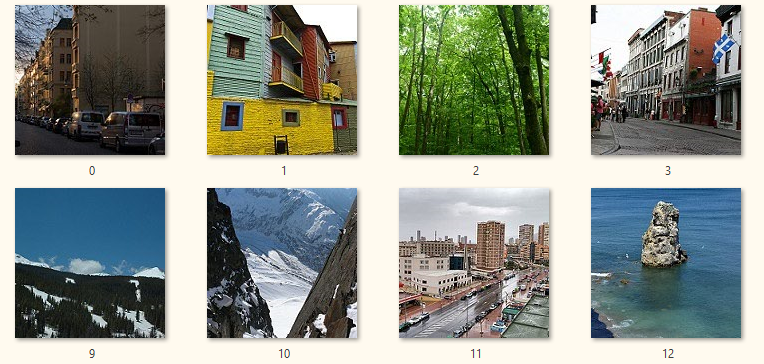
\includegraphics[width=\linewidth]{dataset_color.png}
        \caption{Sample of Color Data Set}
        \label{fig:dataset_color}
    \end{subfigure}
    \quad
    \begin{subfigure}[b]{0.8\columnwidth}
        \centering
        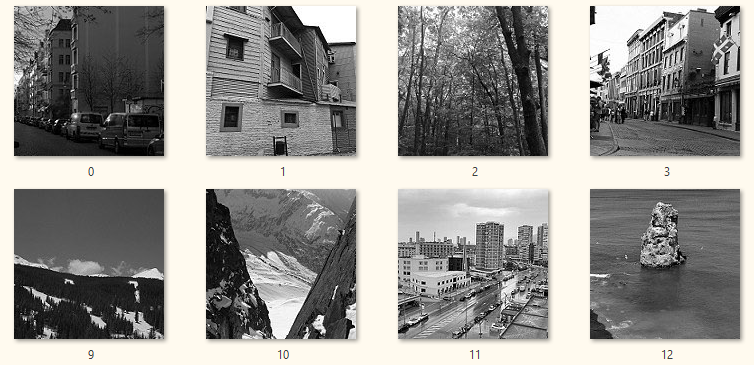
\includegraphics[width=\linewidth]{dataset_gray.png}
        \caption{Sample of Gray-scale Data Set}
        \label{fig:dataset_gray}
    \end{subfigure}
    \caption{Samples of the Dataset Used}
    \label{fig:dataset_samples}
\end{figure}


\item \textbf{Evaluation Metrics:}
During the first milestone, the color mapping techniques mentioned in the \ref{sec:Classical_techniques} were done. The three methods had different PSNR, SSIM values as mentioned in the Table~\ref{table:metrics_results}.

In CNN implementation the model is trained for $20$ and $30$ epochs using the Adam optimizer with a learning rate of $0.001$. Mean Squared Error (MSE) is used as the primary loss function, and the model is evaluated using the following metrics:
\begin{itemize}
    \item \textbf{MSE}: The pixel-wise difference between predicted and ground-truth images is measured. (Used for CNN Model Only)
    \item \textbf{PSNR}: The quality of the predicted images relative to the ground truth is indicated.
    \item \textbf{SSIM}: The structural similarity between predicted and ground-truth images is measured.
    \item \textbf{R²}: How well the predicted colors match the ground truth is measured. (Used for CNN Model Only)
\end{itemize}
\end{itemize}
The average range of evaluation metrics on the validation set are summarized in Table~\ref{table:metrics_results}.

\begin{table}[t]
\centering
\renewcommand{\arraystretch}{1.1} % Adjust row height
\setlength{\tabcolsep}{4pt} % Adjust column spacing
\begin{tabular}{|p{2.5cm}|c|c|p{3.3cm}|}  % Adjust column widths
\hline
\textbf{Method} & \textbf{PSNR} & \textbf{SSIM} & \textbf{Observations} \\ \hline
Intensity-Based Color Mapping & 5 - 7 & 0.01 - 0.3 & Limited color diversity \\ \hline
Custom Color Mapping & 4 - 10 & -0.05 - 0.45 & Better structure preservation relative to Intensity based Mapping \\ \hline
OpenCV Color Mapping & 4 - 9 & 0.4 - 0.6 & Better structure preservation relative to Custom Mapping \\ \hline
CNN Fine-Tuned & \textbf{23.14} & \textbf{0.93} & Most realistic colorization \\ \hline
\end{tabular}
\caption{Comparison of Colorization Techniques}
\label{table:metrics_results}
\end{table}


\subsection{Enhancement}
Strong performance is achieved by the model on the validation set, as evidenced by the quantitative metrics and qualitative results. However, some limitations are observed:
\begin{itemize}
    \item Fine details and textures in complex images are struggled with by the model.
    \item The colorization is observed to appear de-saturated in some cases.
\end{itemize}
The use of perceptual loss improved the visual quality of the predicted images.


\subsection{Quantitative Results}
The numbers for PSNR, SSIM were directly obtained for the classical color mapping techniques. Those values did not depict the expected level of performance.

For the CNN approach, the training loss, loss over R\textsuperscript{2} PSNR, and SSIM curves over $30$ epochs with perceptual loss function integration, are shown in Figure~\ref{fig:training_metrics}. The training loss is observed to be decreased steadily and plateau after $20$ epochs, indicating convergence. The PSNR and SSIM curves are seen to increase steadily, demonstrating that the model improves over time.

\begin{figure}[t]
    \centering
    \begin{subfigure}{\columnwidth}
        \centering
        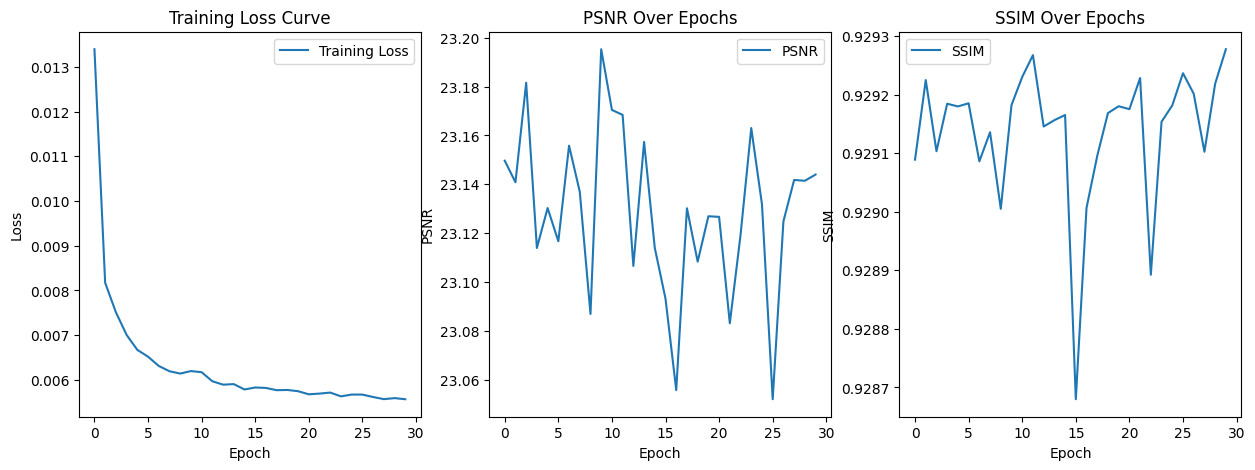
\includegraphics[width=\linewidth]{6_loss_psnr_ssim.png}
        \caption{Training loss, PSNR, and SSIM curves.}
        \label{fig:curves}
    \end{subfigure}
    \hfill
    \begin{subfigure}{\columnwidth}
        \centering
        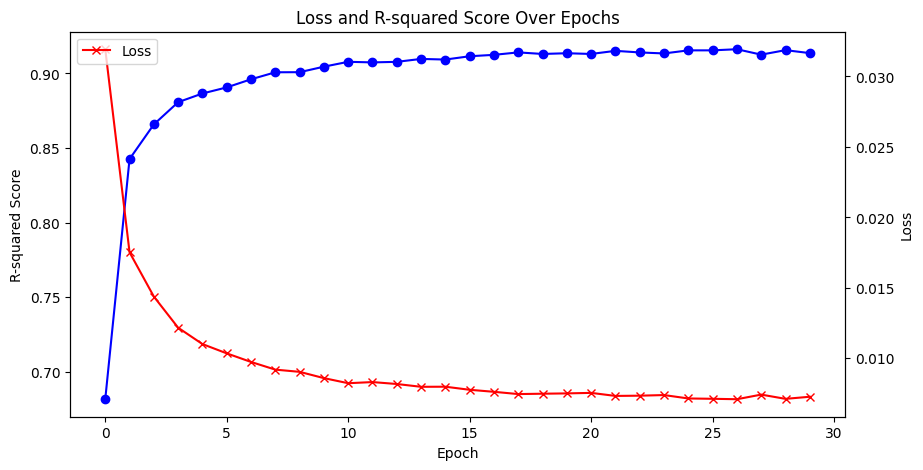
\includegraphics[width=\linewidth]{7_loss_over_Rsquard_score.png}
        \caption{Loss over R\textsuperscript{2} score.}
        \label{fig:loss_r2}
    \end{subfigure}
    \hfill
    \begin{subfigure}{\columnwidth}
        \centering
        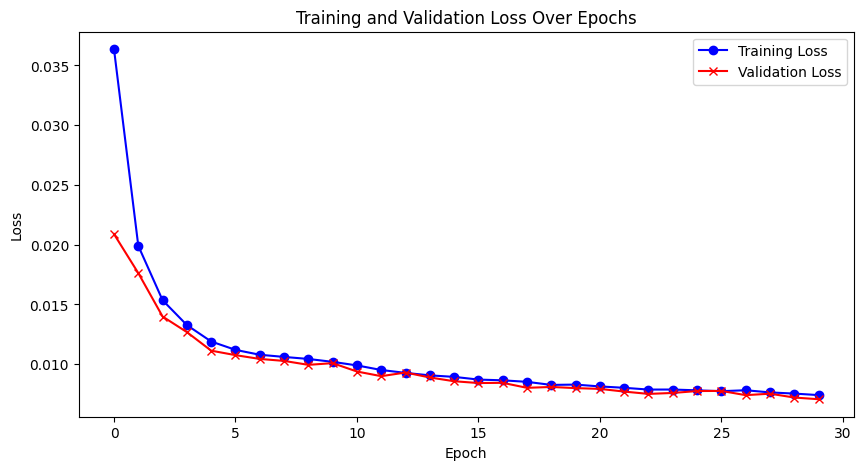
\includegraphics[width=\linewidth]{8_training_loss_validation_loss.png}
        \caption{Training and validation loss.}
        \label{fig:train_val_loss}
    \end{subfigure}
    
    \caption{Training performance metrics over epochs.}
    \label{fig:training_metrics}
\end{figure}


\subsection{Qualitative Results}
Color Mapping technique felt short when it comes to proper colorization, a sample set of results can seen in Figure~\ref{fig:color_mapping_results}.

\begin{figure}[t]
    \centering
    \begin{subfigure}[b]{\linewidth}
        \centering
        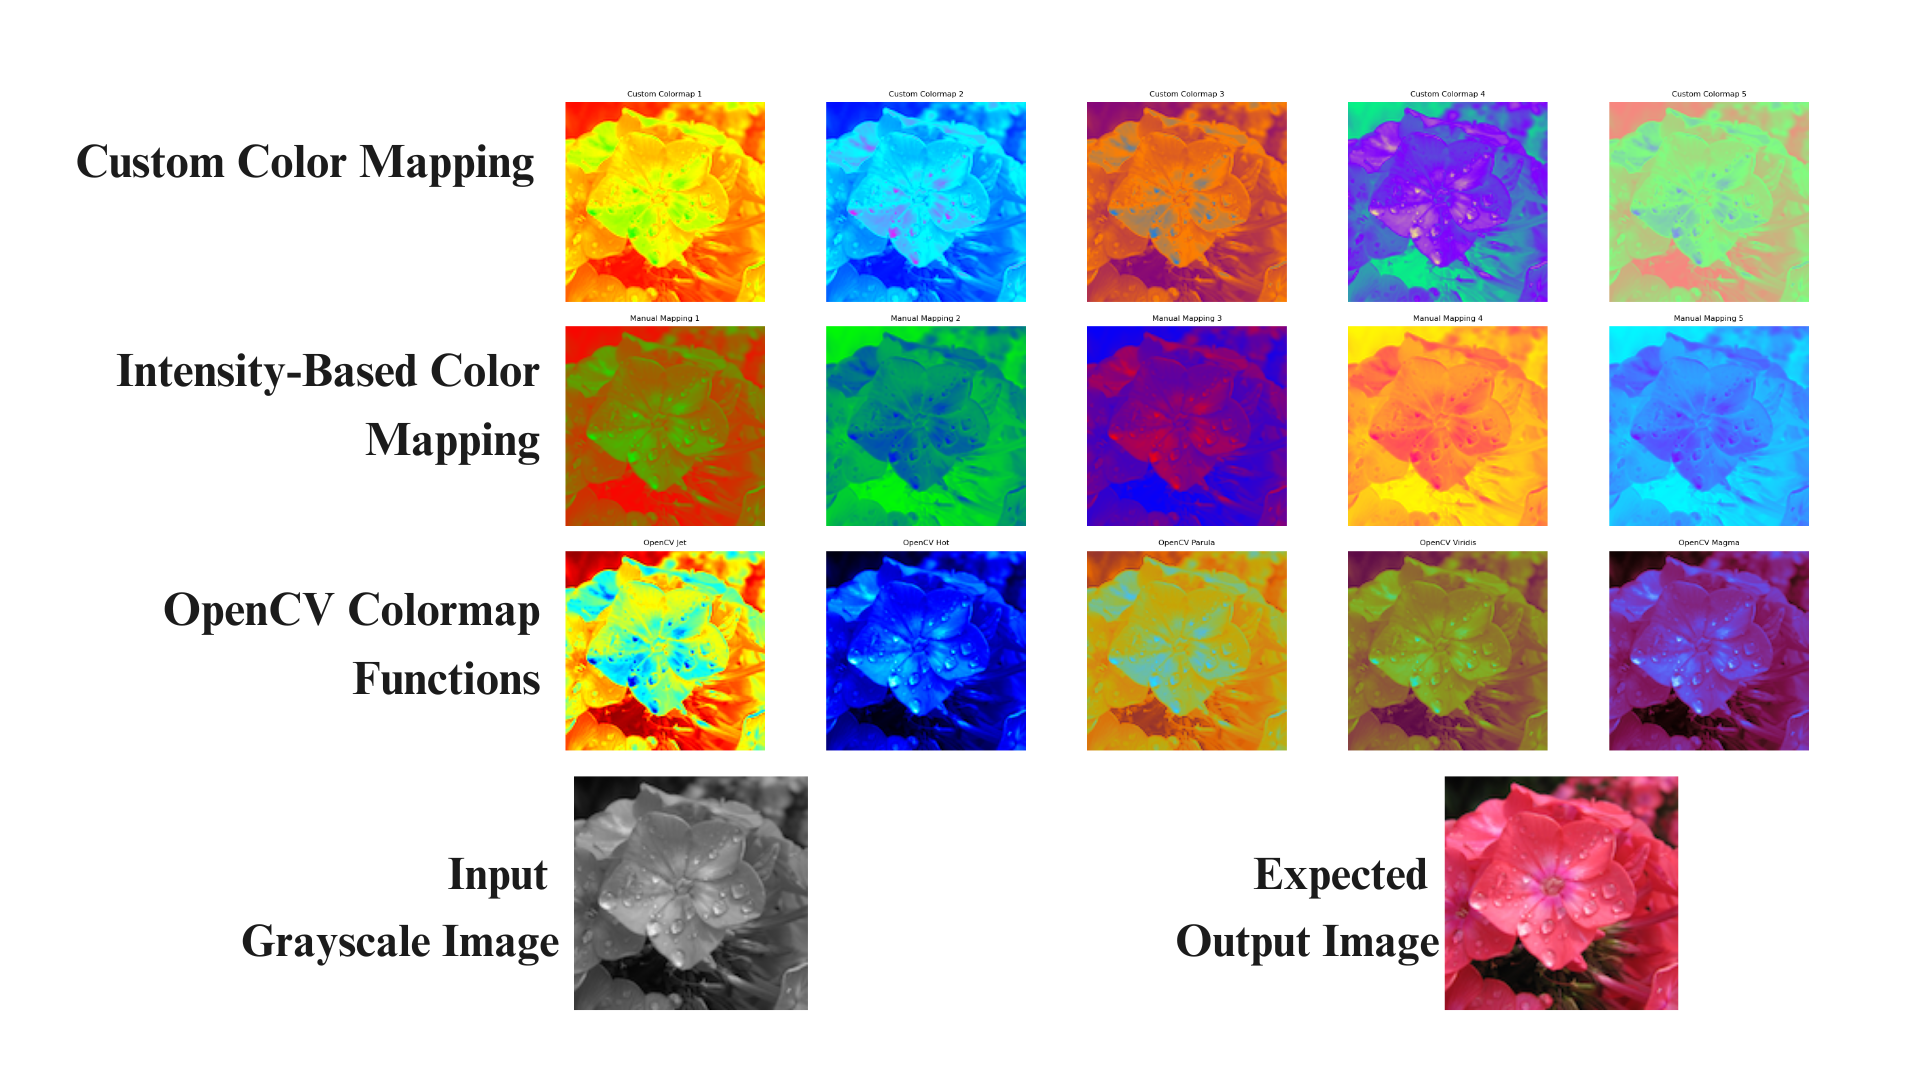
\includegraphics[width=\linewidth]{classical_techniques.png}
        \label{fig:classical_techniques}
    \end{subfigure}
    \hfill
    \begin{subfigure}[b]{\linewidth}
        \centering
        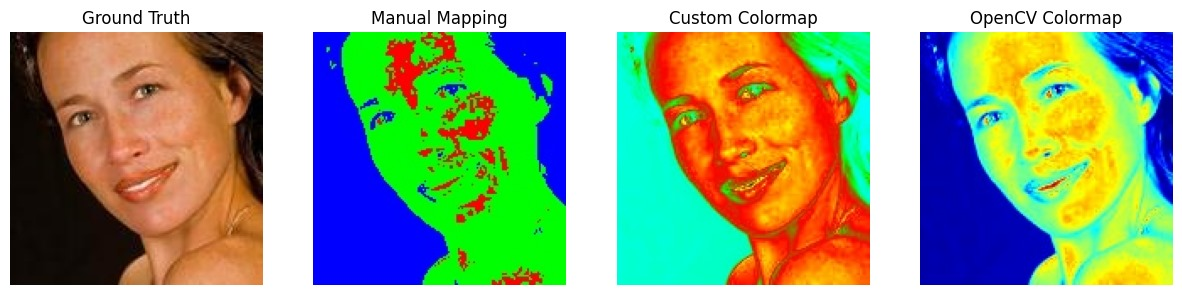
\includegraphics[width=\linewidth]{colormap1.jpg}
        \label{fig:colormap1}
    \end{subfigure}
    \vspace{0.3cm} % Adds vertical spacing between rows
    \begin{subfigure}[b]{\linewidth}
        \centering
        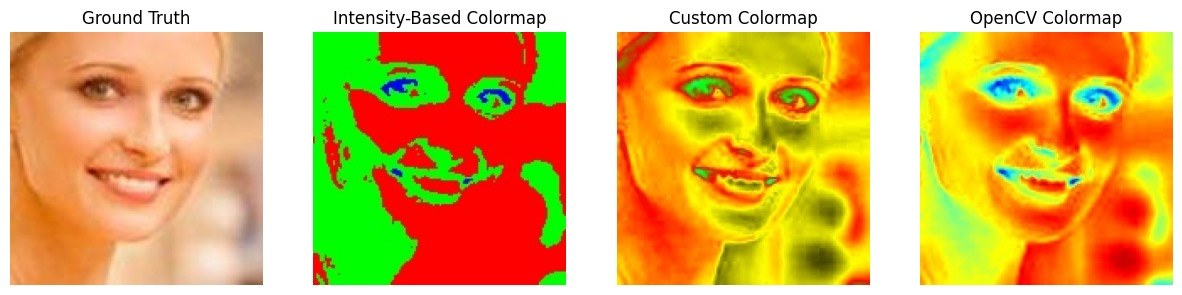
\includegraphics[width=\linewidth]{colormap2.jpg}
        \label{fig:colormap2}
    \end{subfigure}
    \hfill
    \begin{subfigure}[b]{\linewidth}
        \centering
        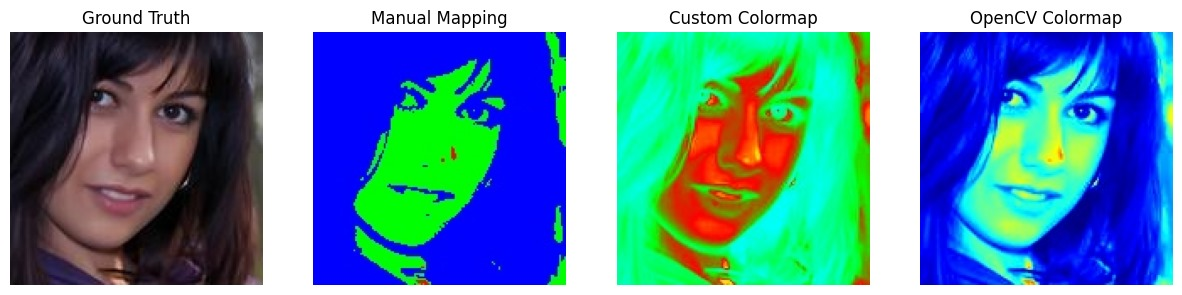
\includegraphics[width=\linewidth]{colormap3.jpg}
        \label{fig:colormap3}
    \end{subfigure} 
    \caption{Example results from Color Mapping Techniques}
    \label{fig:color_mapping_results}
\end{figure}



For the CNN Approach, example results of the model's predictions before and after the integration of perceptual loss function are shown in Figure~\ref{fig:before_perceptual_loss} and Figure~\ref{fig:after_perceptual_loss}. The grayscale input, predicted color image, and ground truth color image are displayed side by side. Plausible colors are successfully predicted for most images, although some fine details are observed to be lost.

\begin{figure}[t]
    \centering
    \begin{subfigure}{\columnwidth}
        \centering
        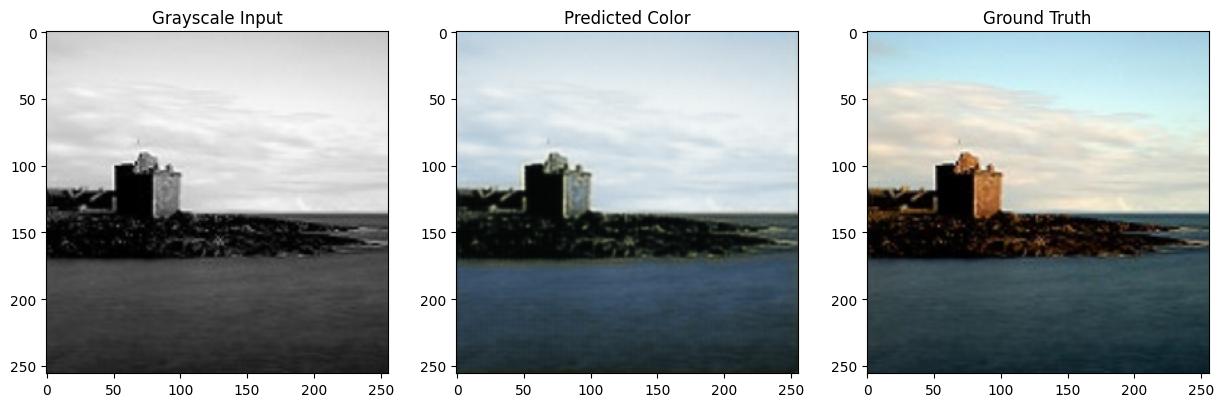
\includegraphics[width=\linewidth]{1_1000dataset_epochs20_result.png}
        \caption{1000 dataset, 20 epochs.}
        \label{fig:1000_20}
    \end{subfigure}
    \hfill
    \begin{subfigure}{\columnwidth}
        \centering
        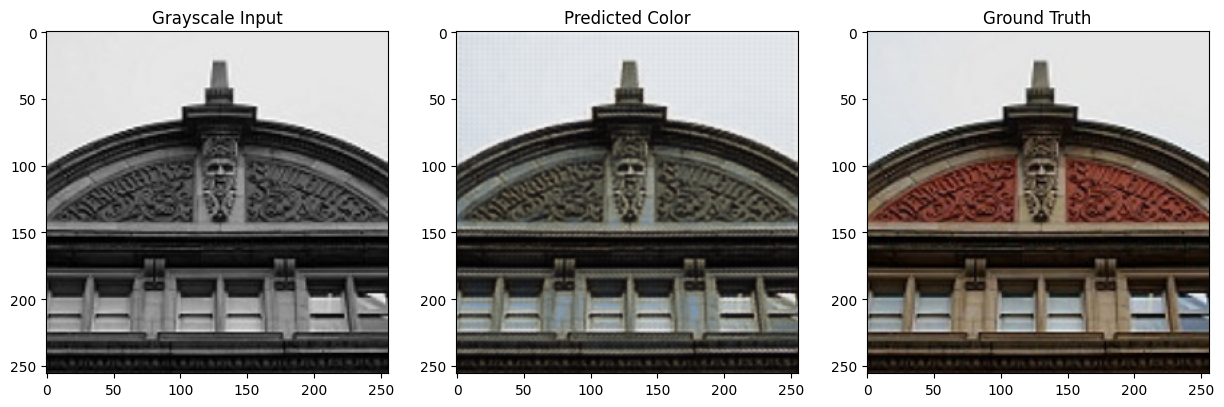
\includegraphics[width=\linewidth]{2_1000dataset_epochs30_result.png}
        \caption{1000 dataset, 30 epochs.}
        \label{fig:1000_30}
    \end{subfigure}
    \hfill
    \begin{subfigure}{\columnwidth}
        \centering
        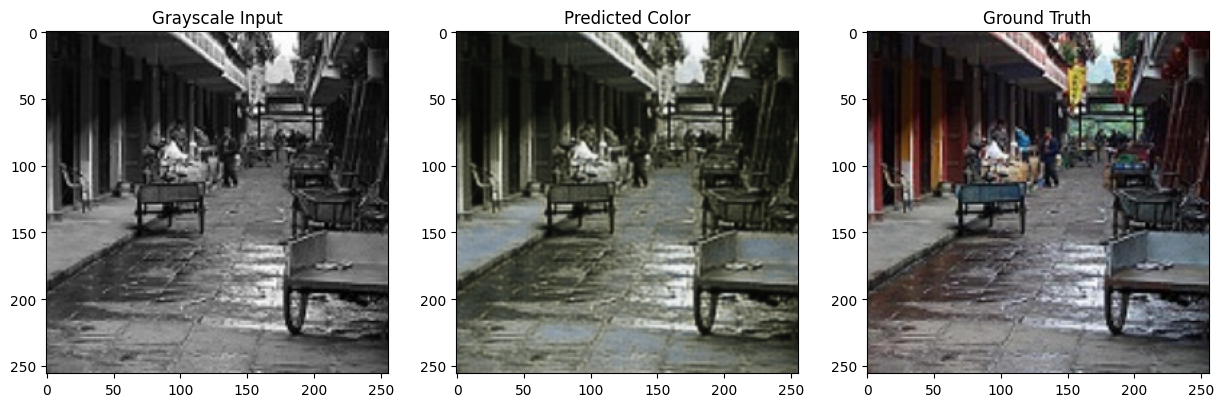
\includegraphics[width=\linewidth]{4_2000dataset_epochs20_result.png}
        \caption{2000 dataset, 20 epochs.}
        \label{fig:2000_20}
    \end{subfigure}

    \caption{Example results before perceptual loss integration: grayscale input (left), predicted color image (middle), and ground truth (right).}
    \label{fig:before_perceptual_loss}
\end{figure}

\begin{figure}[t]
    \centering
    \begin{subfigure}{\columnwidth}
        \centering
        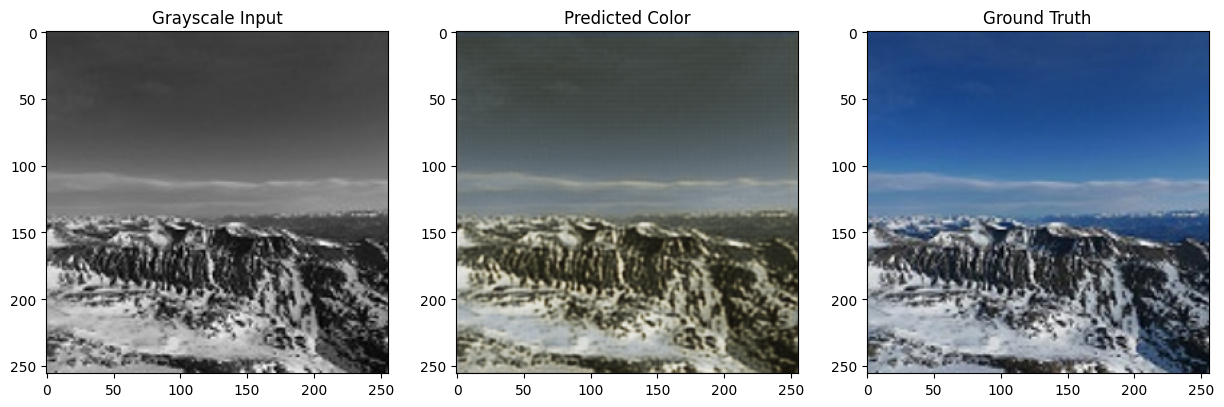
\includegraphics[width=\linewidth]{3_1000dataset_with_perceptual_loss_result.png}
        \caption{1000 dataset with perceptual loss.}
        \label{fig:1000_perceptual}
    \end{subfigure}
    \hfill
    \begin{subfigure}{\columnwidth}
        \centering
        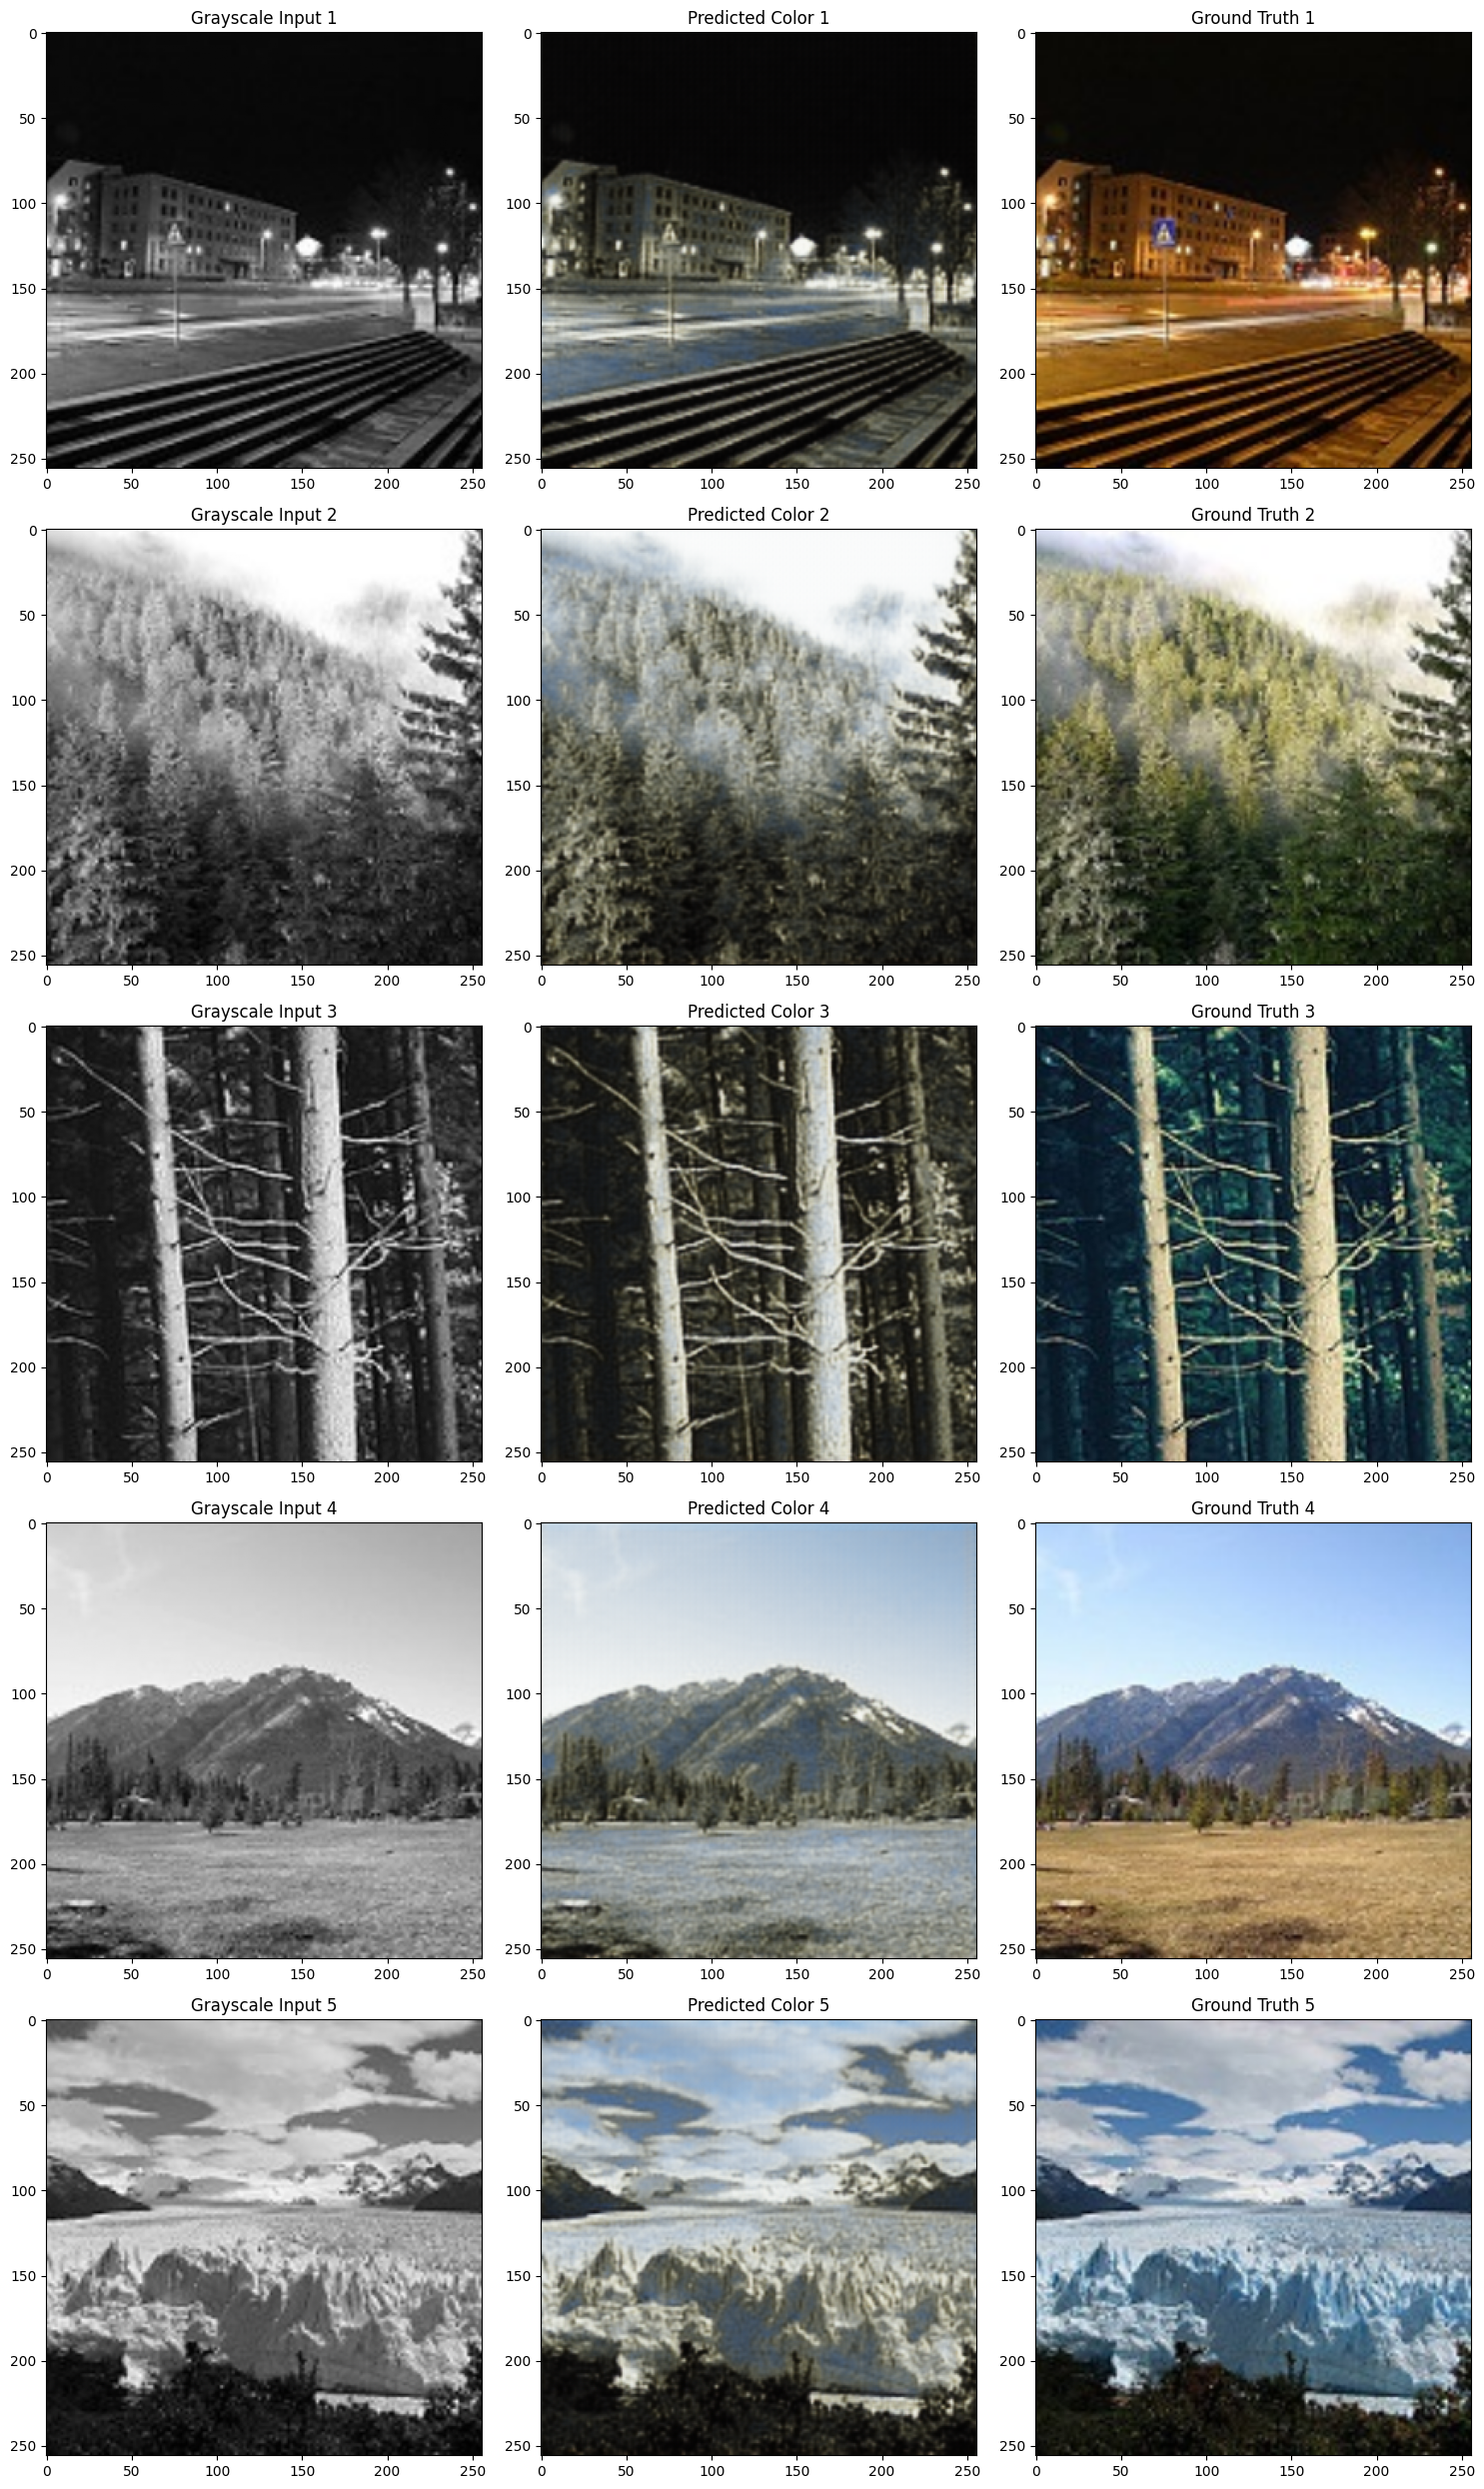
\includegraphics[width=\linewidth]{5_2000dataset_with_perceptual_loss_result.png}
        \caption{2000 dataset with perceptual loss.}
        \label{fig:2000_perceptual}
    \end{subfigure}

    \caption{Example results after perceptual loss integration: grayscale input (left), predicted color image (middle), and ground truth (right).}
    \label{fig:after_perceptual_loss}
\end{figure}




\section{Conclusion}
\subsection{Key Findings}
\begin{itemize}
\item Classical methods are effective for simple textures but struggle with complex objects.
\item CNN-based models significantly improve realism by leveraging learned color distributions.
\item Combining classical preprocessing with CNN training yields superior results.
\end{itemize}

The above findings can be observed when two sample images are loaded upon the methods as in Figure~\ref{fig:colorization_op1} and Figure~\ref{fig:colorization_op2}

\begin{figure}[t]
    \centering
    % CNN Output in a single row
    \subcaptionbox{CNN Approach for Sample 1\label{subfig:CNN_OP1}}{
        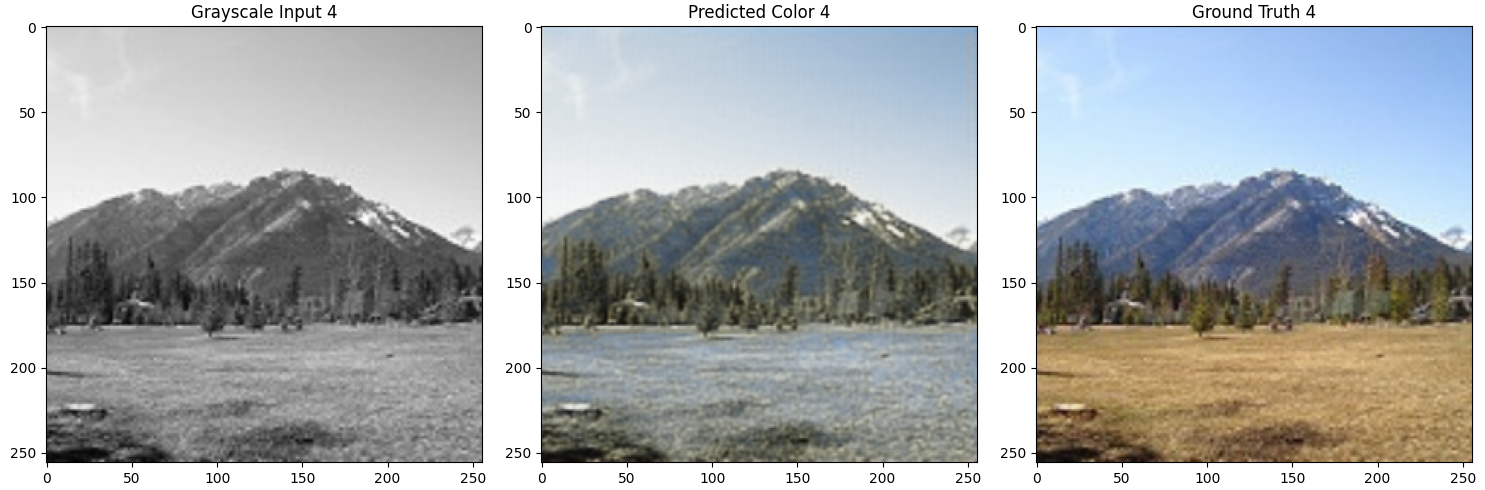
\includegraphics[width=\linewidth]{CNN_OP1.png}
    }
    
    \vspace{0.1cm} % Space between rows

    % Second row - Other three methods
    \subcaptionbox{Custom Color Map for Sample 1\label{subfig:Custom_Color_Map_OP1}}{
        \includegraphics[width=0.29\linewidth]{Custom_Color_Map_OP1.jpg}
    }
    \subcaptionbox{Intensity Based Color Map For Sample 1\label{subfig:Manual_Color_Map_OP1}}{
        \includegraphics[width=0.29\linewidth]{Manual_Color_Map_OP1.jpg}
    }
    \subcaptionbox{OpenCV Color Map For Sample 1\label{subfig:OpenCV_Color_Map_OP1}}{
        \includegraphics[width=0.29\linewidth]{OpenCV_Color_Map_OP1.jpg}
    }

    \caption{Comparison of different colorization methods for Sample 1}
    \label{fig:colorization_op1}
\end{figure}

\begin{figure}[b]
    \centering
    % CNN Output in a single row
    \subcaptionbox{CNN Approach for Sample 2\label{subfig:CNN_OP2}}{
        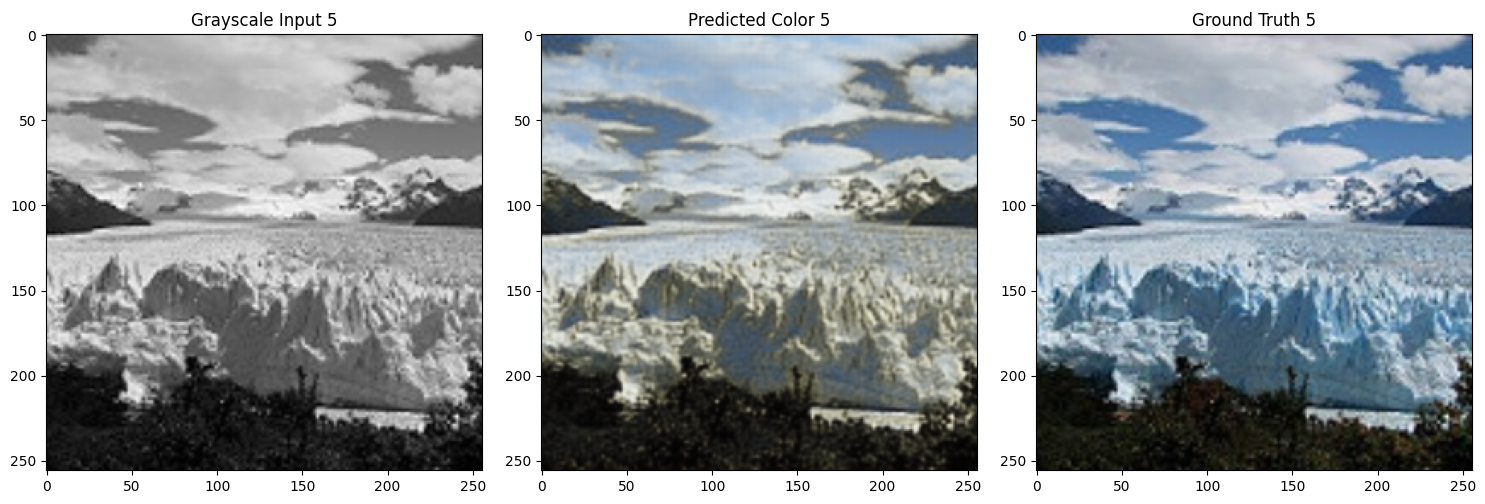
\includegraphics[width=\linewidth]{CNN_OP2.png}
    }
    
    \vspace{0.1cm} % Space between rows

    % Second row - Other three methods
    \subcaptionbox{Custom Color Map For Sample 2\label{subfig:Custom_Color_Map_OP2}}{
        \includegraphics[width=0.29\linewidth]{Custom_Color_Map_OP2.jpg}
    }
    \subcaptionbox{Intensity Color Map For Sample 2\label{subfig:Manual_Color_Map_OP2}}{
        \includegraphics[width=0.29\linewidth]{Manual_Color_Map_OP2.jpg}
    }
    \subcaptionbox{OpenCV Color Map For Sample 2\label{subfig:OpenCV_Color_Map_OP2}}{
        \includegraphics[width=0.29\linewidth]{OpenCV_Color_Map_OP2.jpg}
    }

    \caption{Comparison of different colorization methods for Sample 2.}
    \label{fig:colorization_op2}
\end{figure}



\subsection{Future Work}
\begin{itemize}
    \item \textbf{Real-Time Implementation:} Optimize the model for video-based colorization by leveraging temporal consistency between frames. This could involve using recurrent neural networks (RNNs) or temporal convolutional networks (TCNs) to handle the sequence of frames efficiently, ensuring smooth and consistent colorization in real-time applications.
    \item \textbf{Dataset Expansion:} Train the model on a larger and more diverse dataset, incorporating a variety of image types, lighting conditions, and textures to improve the model's generalizability and robustness. Using high-quality and high-resolution datasets will allow the model to better handle a wider range of images and edge cases.
    \item \textbf{Adaptive Learning:} Implement reinforcement learning techniques to enable continuous improvement of the model. By incorporating a feedback loop where the model evaluates its predictions and adjusts its parameters based on user feedback or quality metrics, it can progressively enhance its performance in real-world applications.
    \item \textbf{Adversarial Learning:} Explore the use of Generative Adversarial Networks (GANs) to enhance the realism and detail of the colorized images. A GAN-based approach could involve training a discriminator to distinguish between real and generated colorized images, pushing the generator to produce more realistic and high-quality colorizations, especially for challenging or ambiguous regions.
\end{itemize}


\begin{thebibliography}{99}
\bibitem{levin2004colorization} A. Levin, D. Lischinski, and Y. Weiss, “Colorization using Optimization,” ACM Transactions on Graphics, vol. 23, no. 3, pp. 689–694, 2004.
\bibitem{gao2019fourier} S. Gao, M. Zhang, et al., “Fourier Transform-based Image Enhancement Techniques,” IEEE Transactions on Image Processing, vol. 28, no. 5, pp. 2169-2181, 2019.
\bibitem{zhang2016colorful} R. Zhang, P. Isola, and A. A. Efros, “Colorful Image Colorization,” ECCV, 2016.
\bibitem{antic2019deoldify} J. Antic, “DeOldify: A Deep Learning-Based Project for Colorizing and Restoring Old Images,” 2019. [Online]. Available: https://github.com/jantic/DeOldify
\bibitem{isola2017image} P. Isola, J. Zhu, T. Zhou, and A. A. Efros, “Image-to-Image Translation with Conditional Adversarial Networks,” CVPR, 2017.
\end{thebibliography}
\vspace{12pt}
\end{document}
